\section{Heat demand prediction model using machine learning.}

This chapter will summarize report of the minor project students from big data module.
There are 2 data sets had been used. One of these data sets was delivered by a member of HAN. It contains the weekly heat production of a house with a heat pump and a gas heating. This data set would provide the information about the heat demand, the output of the model. The other data set used was the weather data of the closest weather station (Instituut, 2019). This data set would provide the inputs to the model, consisting of the average weekly temperature, the average weekly wind speed, the average weekly sunshine duration the overall sum of sunshine duration, the average hourly precipitation and the sum of precipitation per week. This data was gained from hourly values provided by the Dutch weather service.\\
The heat production data was manually cleaned to get rid of outliers, measurement errors and other unwanted values. Dimensions of each column were checked, gaps filled and intervals between data checked for uniformity. As the heat production was given as an accumulative sum, the heat production per week needed to be extracted.
The data was split to 70${\%}$ for training and 30${\%}$ for testing.
As the NN was doing classification in the assignment, the evaluation had to be changed as well. New error metrics for this prediction model had to be established. Mean absolute Error, mean absolute relative error and mean absolute percentage error are a few to name.

\subsection{Neural Network MATLAB toolbox.}

The NN MATLAB toolbox for neural fitting was applied to the data. This toolbox applies a 2-layer feed-forward network with sigmoid hidden neurons and linear output neurons (figures \ref{fig:NNMatlb}). 

\begin{figure}[H]
	\centering
	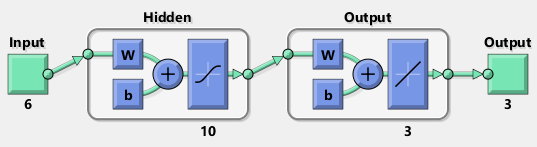
\includegraphics[width=1.0\columnwidth]{Pictures/NN matlab.png}
	\caption[Short title]{NN as used by the neural fitting toolbox}
	\label{fig:NNMatlb}
	\end{figure}

This network is then fed with the $x_{train}$ and $y_{train}$ previously generated for the manual implementation of the NN (figure \ref{fig:NNinput}). 

\begin{figure}[H]
	\centering
	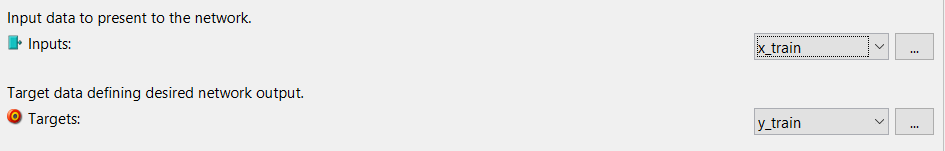
\includegraphics[width=1.0\columnwidth]{Pictures/Input to NN.png}
	\caption[Short title]{Input to NN}
	\label{fig:NNinput}
	\end{figure}

The training data set is then split up into training- test- and validation- set (figure \ref{fig:Trainingvs}). This splitting cannot be reduced to zero. As it is a toolbox function, the validation and test data set were part of the overall training algorithm, so the values were not changed. This data splitting is unconnected to the initial splitting between test and validation set. Here the training data set is internally split up by the toolbox.

\begin{figure}[H]
	\centering
	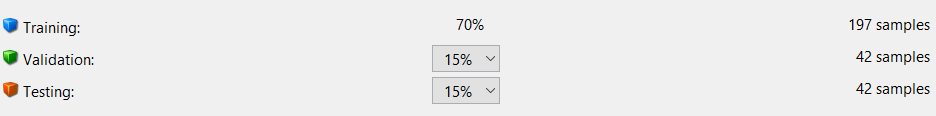
\includegraphics[width=1.0\columnwidth]{Pictures/Training data vs Validation and Testing data ratio.png}
	\caption[Short title]{Training data vs Validation and Testing data ratio}
	\label{fig:Trainingvs}
	\end{figure}

For the hidden layer 10 neurons are chosen.

From the validation performance (figure \ref{fig:Validation Performance}), it can be clearly seen, that the NN is being trained quickly. By the validation performance it is determined, that at epoch 17 the NN delivers best performance so training can be stopped.

\begin{figure}[H]
	\centering
	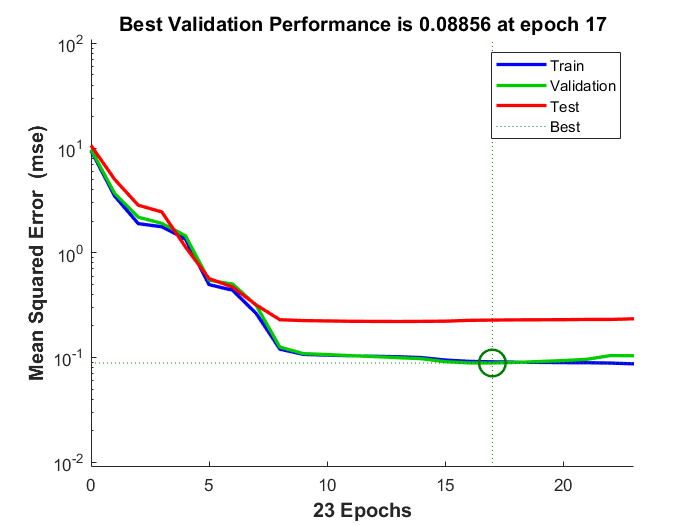
\includegraphics[width=1.0\columnwidth]{Pictures/Validation Performance.png}
	\caption[Short title]{Validation Performance}
	\label{fig:Validation Performance}
	\end{figure}
	
The MSE (mean squared error) can be found in the table \ref{tab:Minimumheat}.

\begin{table}[H]
    \centering
    \begin{tabular}{|c|c|c|}
    \hline
    MSE (norm) & Training Data & Test data \\
    
    \hline
     Heat Pump     &  0.144817 & 0.593376\\
     
     \hline
     Gas           &  0.044751 & 0.218106\\
     
     \hline
     Combine       &  0.136688   & 0.586856\\
    \hline


    \end{tabular}
    \caption{Minimum heating powercapacity}
    \label{tab:Minimumheat}
\end{table}

\subsection{Regression MATLAB toolbox}

The regression SVM toolbox in MATLAB was employed. Using the regression model through SVM  (Gaussian kernel) function, the root mean square error (RMSE) is very small and so are the other error metrics.  A 5-fold cross validation is used to validate the model (figure \ref{fig:k-fold cross validation}).\\
Cross validation is also called a rotation estimation. It’s very easy to see how accurately the predictive model will perform in practical settings. The data is divided into 5 portions of test data sets and training data sets for each iteration. The same test set is not used for all iterations. This testing is just an internal metric of the toolbox and can be seen as part of the training algorithm. It is independent of the initial splitting into test and training data. The cross validation is purely run on the training data. This cross validation is part of the toolbox and can’t be removed.


\begin{figure}[H]
	\centering
	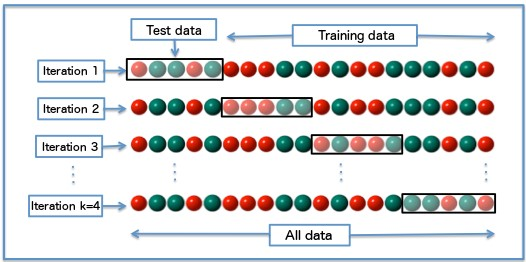
\includegraphics[width=1.0\columnwidth]{Pictures/k-fold cross validation.jpg}
	\caption[Short title]{k-fold cross validation}
	\label{fig:k-fold cross validation}
	\end{figure}
	
The MSE is shown in the table \ref{tab:Minimumheatpower}.

\begin{table}[H]
    \centering
    \begin{tabular}{|c|c|c|}
    \hline
    MSE (norm) & Training Data & Test data \\
    
    \hline
     Heat Pump     &  0.178197 & 0.238478\\
     
     \hline
     Gas           &  0.060874 & 	0.249772\\
     
     \hline
     Combine       &  0.167937   & 0.245215\\
    \hline


    \end{tabular}
    \caption{Minimum heating powercapacity}
    \label{tab:Minimumheatpower}
\end{table}

In the figure \ref{fig:Predicvsactual_temp}, the graph corresponds to the actual heat production and the predicted heat production as given by the toolbox. It can be seen here that there is a good correlation between the output (heat demand) and the temperature (x-axis, $column_{1}$).

\begin{figure}[H]
	\centering
	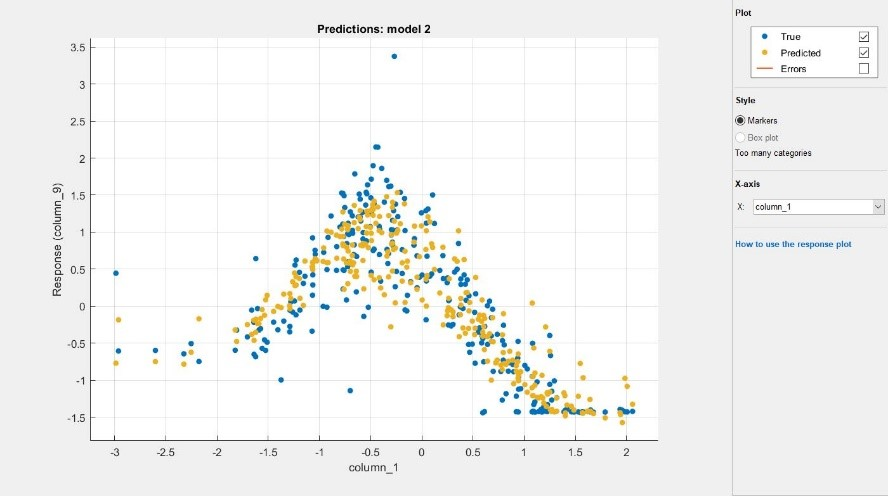
\includegraphics[width=1.0\columnwidth]{Pictures/predicvsheardemand temp.jpg}
	\caption[Short title]{Predicted vs actual heat demand based on temperature}
	\label{fig:Predicvsactual_temp}
	\end{figure}
	
From the simulation results it could be seen that the data gives enough information for prediction. An improvement on the data set would provide better results with any prediction method.
The SVM with the regression toolbox can find a correlation in the data, especially with the temperature input. The MSE for the SVM are even better than the ones of the neural network generated with the toolbox. Also, the MSE on the test data is best for the SVM generated with the regression toolbox. Although it needs training for each output individually, the SVM gives the best predictions.

\newpage
	
	
